
\documentclass[a4paper,12pt]{scrbook}
\usepackage{amsmath,amssymb,amsthm}
\usepackage{fancyvrb}
\usepackage{parskip}
\usepackage{lastpage}
\usepackage{verbatim,boxedminipage,enumitem}
\usepackage{ifthen}
\usepackage{color,graphicx}
\usepackage{pgf}
\usepackage{longtable}
\usepackage{upquote}
%\usepackage[all]{xy}
\usepackage{tobiShell}
\usepackage{tikz}
\usetikzlibrary{automata}
\usetikzlibrary{arrows}
\usepackage{pgf,pgfarrows,pgfnodes}
\usepackage{pgfplots}
\usepackage{circuitikz}
\usetikzlibrary{circuits}
\usetikzlibrary{circuits.logic.US}
\usepackage{mymath}
\usepackage{python}
%------------------------------------------------------------------
% Verbatim for console window - single line frame, no line numbers
%------------------------------------------------------------------
\DefineVerbatimEnvironment%
 {console}{Verbatim}
 {frame=single}

%--------------------------------------------------------
% Remove the vertical spacing before and after Verbatim.
%--------------------------------------------------------
\usepackage{atbeginend}
\BeforeBegin{console}{\mbox{}\\ \begin{minipage}{\textwidth}\vspace{3pt}}
\AfterEnd{console}{\vspace{4pt} \end{minipage} \\ }

\begin{document}
\thispagestyle{empty}

\begin{center}
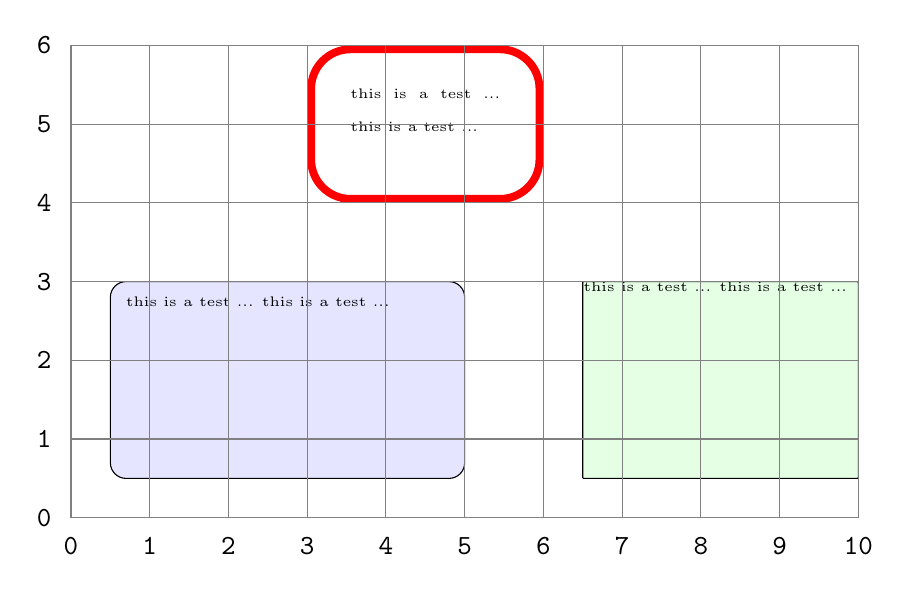
\begin{tikzpicture}

\draw (4.5, 5.0)
  node[draw, line width=0.1cm, , color=red,
       rounded corners=0.5cm, inner sep=0.5cm] {

\begin{minipage}[t][0.9cm]{1.9cm}
\mbox{}

\end{minipage}

};
\draw (4.5, 5.0) node[color=black,
 inner sep=0.5cm] {
 
\begin{minipage}[t][0.9cm]{1.9cm}
{\tiny this is a test ... this is a test ...}
\end{minipage}

};
\draw (2.75, 1.75)
  node[fill=blue!10!white,rounded corners=0.2cm,inner sep=0.2cm] {

\begin{minipage}[t][2.1cm]{4.1cm}
\mbox{}

\end{minipage}

};
\draw (2.75, 1.75)
  node[draw, , , color=black,
       rounded corners=0.2cm, inner sep=0.2cm] {

\begin{minipage}[t][2.1cm]{4.1cm}
\mbox{}

\end{minipage}

};
\draw (2.75, 1.75) node[color=black,
 inner sep=0.2cm] {
 
\begin{minipage}[t][2.1cm]{4.1cm}
{\tiny this is a test ... this is a test ...}
\end{minipage}

};
\draw (8.25, 1.75)
  node[fill=green!10!white,rounded corners=0.01cm,inner sep=0.01cm] {

\begin{minipage}[t][2.48cm]{3.48cm}
\mbox{}

\end{minipage}

};
\draw (8.25, 1.75)
  node[draw, , , color=black,
       rounded corners=0.01cm, inner sep=0.01cm] {

\begin{minipage}[t][2.48cm]{3.48cm}
\mbox{}

\end{minipage}

};
\draw (8.25, 1.75) node[color=black,
 inner sep=0.01cm] {
 
\begin{minipage}[t][2.48cm]{3.48cm}
{\tiny this is a test ... this is a test ...}
\end{minipage}

};\draw[gray] (0.0,0.0) -- (0.0,6);
\draw[gray] (1.0,0.0) -- (1.0,6);
\draw[gray] (2.0,0.0) -- (2.0,6);
\draw[gray] (3.0,0.0) -- (3.0,6);
\draw[gray] (4.0,0.0) -- (4.0,6);
\draw[gray] (5.0,0.0) -- (5.0,6);
\draw[gray] (6.0,0.0) -- (6.0,6);
\draw[gray] (7.0,0.0) -- (7.0,6);
\draw[gray] (8.0,0.0) -- (8.0,6);
\draw[gray] (9.0,0.0) -- (9.0,6);
\draw[gray] (10.0,0.0) -- (10.0,6);
\draw[gray] (0.0,0.0) -- (10,0.0);
\draw[gray] (0.0,1.0) -- (10,1.0);
\draw[gray] (0.0,2.0) -- (10,2.0);
\draw[gray] (0.0,3.0) -- (10,3.0);
\draw[gray] (0.0,4.0) -- (10,4.0);
\draw[gray] (0.0,5.0) -- (10,5.0);
\draw[gray] (0.0,6.0) -- (10,6.0);
\draw(0, 0) node [font=\ttfamily, label=below:{\texttt{0}}] {};
\draw(1, 0) node [font=\ttfamily, label=below:{\texttt{1}}] {};
\draw(2, 0) node [font=\ttfamily, label=below:{\texttt{2}}] {};
\draw(3, 0) node [font=\ttfamily, label=below:{\texttt{3}}] {};
\draw(4, 0) node [font=\ttfamily, label=below:{\texttt{4}}] {};
\draw(5, 0) node [font=\ttfamily, label=below:{\texttt{5}}] {};
\draw(6, 0) node [font=\ttfamily, label=below:{\texttt{6}}] {};
\draw(7, 0) node [font=\ttfamily, label=below:{\texttt{7}}] {};
\draw(8, 0) node [font=\ttfamily, label=below:{\texttt{8}}] {};
\draw(9, 0) node [font=\ttfamily, label=below:{\texttt{9}}] {};
\draw(10, 0) node [font=\ttfamily, label=below:{\texttt{10}}] {};
\draw(0, 0) node [font=\ttfamily, label=left:{\texttt{0}}] {};
\draw(0, 1) node [font=\ttfamily, label=left:{\texttt{1}}] {};
\draw(0, 2) node [font=\ttfamily, label=left:{\texttt{2}}] {};
\draw(0, 3) node [font=\ttfamily, label=left:{\texttt{3}}] {};
\draw(0, 4) node [font=\ttfamily, label=left:{\texttt{4}}] {};
\draw(0, 5) node [font=\ttfamily, label=left:{\texttt{5}}] {};
\draw(0, 6) node [font=\ttfamily, label=left:{\texttt{6}}] {};
\end{tikzpicture}

\end{center}

\end{document}
